Dans cette partie nous allons exposer les principes algorithmiques qui sous-tendent le fonctionnement du résolveur. Cette approche, bien que dénuée de détails techniques et autres soucis d’implémentation, proposera une réponse à nos différents objectifs tout en tenant compte de certaines des contraintes citées précédemment.  Nous nous baserons ici sur la résolution d’un cube 3x3x3 à l’aide du serpent présenté précédemment, le Cubra Orange.

\section{Quelques définitions}

Tout d’abord, deux éléments constituent la base de l’algorithme de résolution :\newline

\begin{itemize}
 \item le serpent, ici le Cubra Orange, composé de 27 unités reliées entre elles
 \item le volume final, ici un cube 3x3x3
\end{itemize}

\vspace{0.5cm}

Le volume final est définit par ses coordonnées, fixées, dans l’espace. Le serpent est quant à lui définit par sa forme qui découle de la nature de chacune des unités qui le composent. En effet, il faut distinguer trois types d’unité du serpent (Figure~\ref{snakeUnits}) :\newline

\begin{itemize}
 \item \textcolor{red}{les extrémités}
 \item \textcolor{blue}{les unités droites}
 \item \textcolor{green}{les coins}
\end{itemize}

\begin{figure}[h]
 \centering
 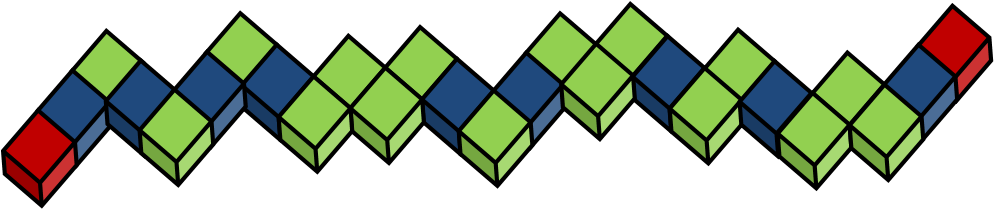
\includegraphics[scale=0.5,keepaspectratio=true]{img/unitTypes.png}
 \caption{Natures des unités du Cubra Orange}
 \label{snakeUnits}
\end{figure}

\clearpage
\section{Construction d’un arbre n-aire}\label{solveNode}
La résolution s’effectue de manière linéaire, en considérant tour à tour chacune des unités du serpent. Le principe est de placer temporairement l’unité considérée à l’intérieur du volume final en fonction de l’emplacement et de la nature de l’unité précédente. On construit ainsi une branche d’un arbre n-aire qui est le cœur de l’algorithme de résolution. Chaque nœud correspond à une unité associée à un couple coordonnées-direction.

Ici il est important de comprendre que ce travail s’effectue de telle sorte que chaque nouvelle unité soit nécessairement placée à l’intérieur du volume final. En tenant compte de cette contrainte et en fonction des emplacements choisis précédemment, on peut constater deux comportements pour une branche donnée. 

Soit on arrive à une impasse, c’est-à-dire qu’une configuration donnée ne permet pas de placer l’unité suivante sans sortir du volume ou la placer sur une autre unité. Dans ce cas, la branche avorte, il faut alors remonter dans l’arborescence jusqu’au prochain nœud qui a donné plusieurs fils. Ce cas de figure est illustré sur les figures~\ref{pathAbort} et~\ref{pathAfter}. Les flèches horizontales représentent les liens de fraternité dans l’arborescence et les flèches verticales représentent les liens de paternité. Ici on a construit six vecteurs initiaux, c’est-à-dire les couples coordonnées-direction possibles pour la première unité. Puis le premier nœud est devenu le nœud courant et a lui-même engendré des fils, en fonction des vecteurs possibles pour la deuxième unité. Et ainsi de suite jusqu’à ce que le nœud représenté en rouge devienne le nœud courant. À ce stade, on admet que ce nœud ne puisse pas engendrer de fils pour une des raisons évoquées précédemment. Cette branche va donc avorter. On va supprimer le nœud rouge et remonter jusqu’à son père (en vert). Si celui-ci a un frère, comme c’est le cas ici avec le nœud bleu, c’est ce frère qui devient le nouveau nœud courant. Il convient de supprimer également le nœud vert qui a généré le sous arbre menant à une impasse.  Ensuite la résolution peut suivre son court, et le nœud bleu générera à son tour ses fils (figure~\ref{pathAfter}).

\begin{figure}[h]
 \centering
 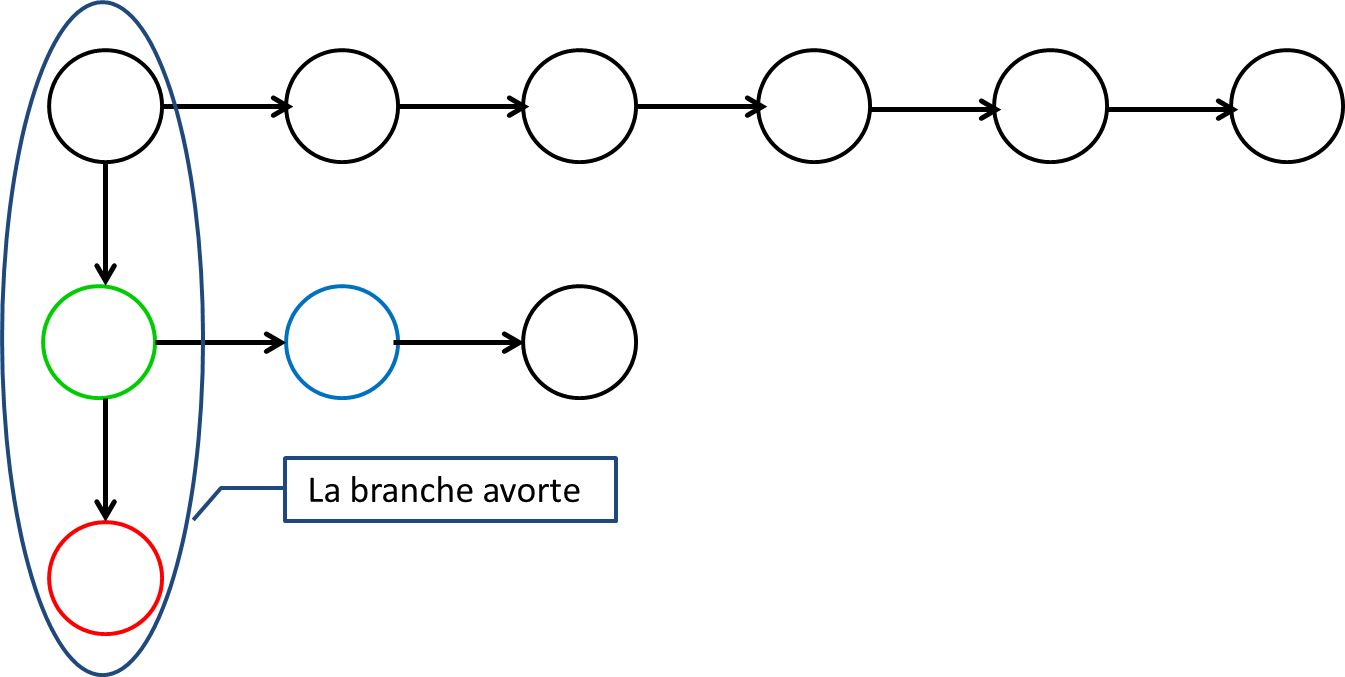
\includegraphics[scale=0.3,keepaspectratio=true]{img/pathAbort.png}
 \caption{Exemple d'une branche qui avorte}
 \label{pathAbort}
\end{figure}

\newpage

\begin{figure}[h]
 \centering
 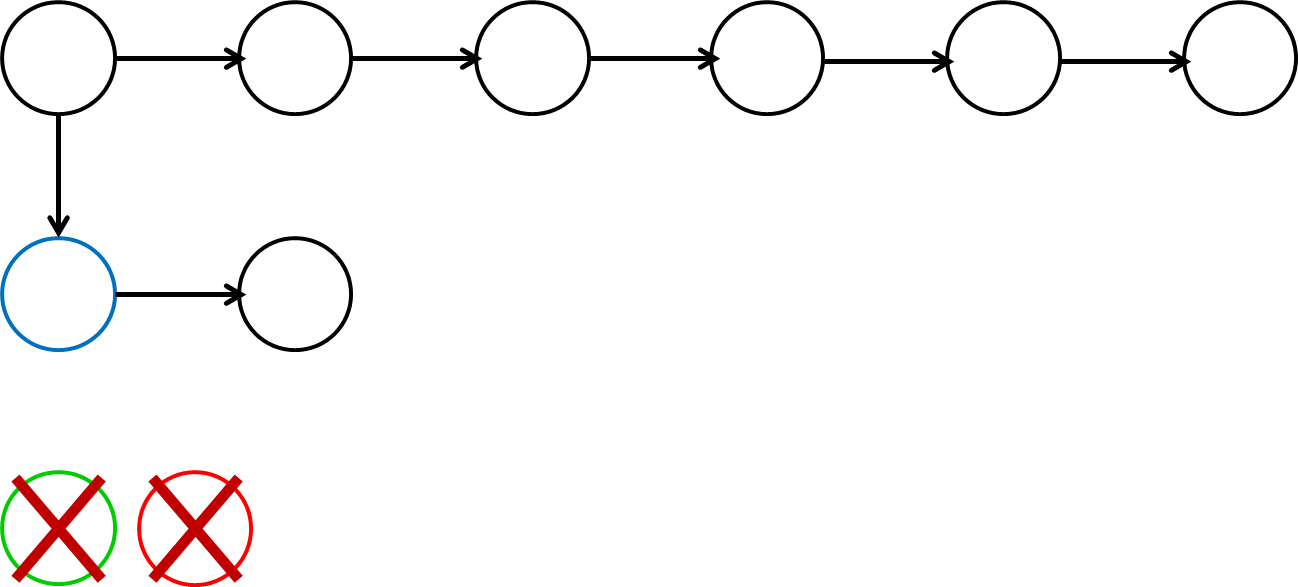
\includegraphics[scale=0.3,keepaspectratio=true]{img/pathAfter.png}
 \caption{Arbre après modifications}
 \label{pathAfter}
\end{figure}

Le deuxième cas de figure est celui où l’on réussit à placer toutes les unités du serpent à l’intérieur du volume. Dans ce cas, la branche aboutit et la succession de ses nœuds depuis la racine constitue une solution au problème. Il faut alors garder cette solution en mémoire puis, comme dans le cas précédent, remonter dans l’arborescence pour chercher des solutions supplémentaires. 

\section{Méthode de calcul des couples coordonnées-direction des nœuds fils}
Lorsqu’un nœud devient le nœud courant, il convient que ses fils soient générés dans l’arbre. Cela consiste notamment à leur attribuer un couple coordonnées-direction dans l’espace. Ce qu’il faut voir ici, c’est que le résultat de cette opération découle de la nature du nœud fils et du couple coordonnées-direction du père. Dans la suite de cette partie, on se placera dans un repère orthonormé (O ; x, y, z). 
Pour calculer les coordonnées des fils d’un nœud, il suffit d’ajouter ses coordonnées avec sa direction. La figure suivante illustre ce procédé. Le nœud marron est le nœud courant et le nœud blanc est son fils. Les coordonnées du fils découlent de la position du père ainsi que de sa direction, matérialisée par la flèche marron. On constate alors que, pour un nœud père donné, tous les fils qu’il va engendrer auront le même triplet de coordonnées dans l’espace. 

\begin{figure}[h]
 \centering
 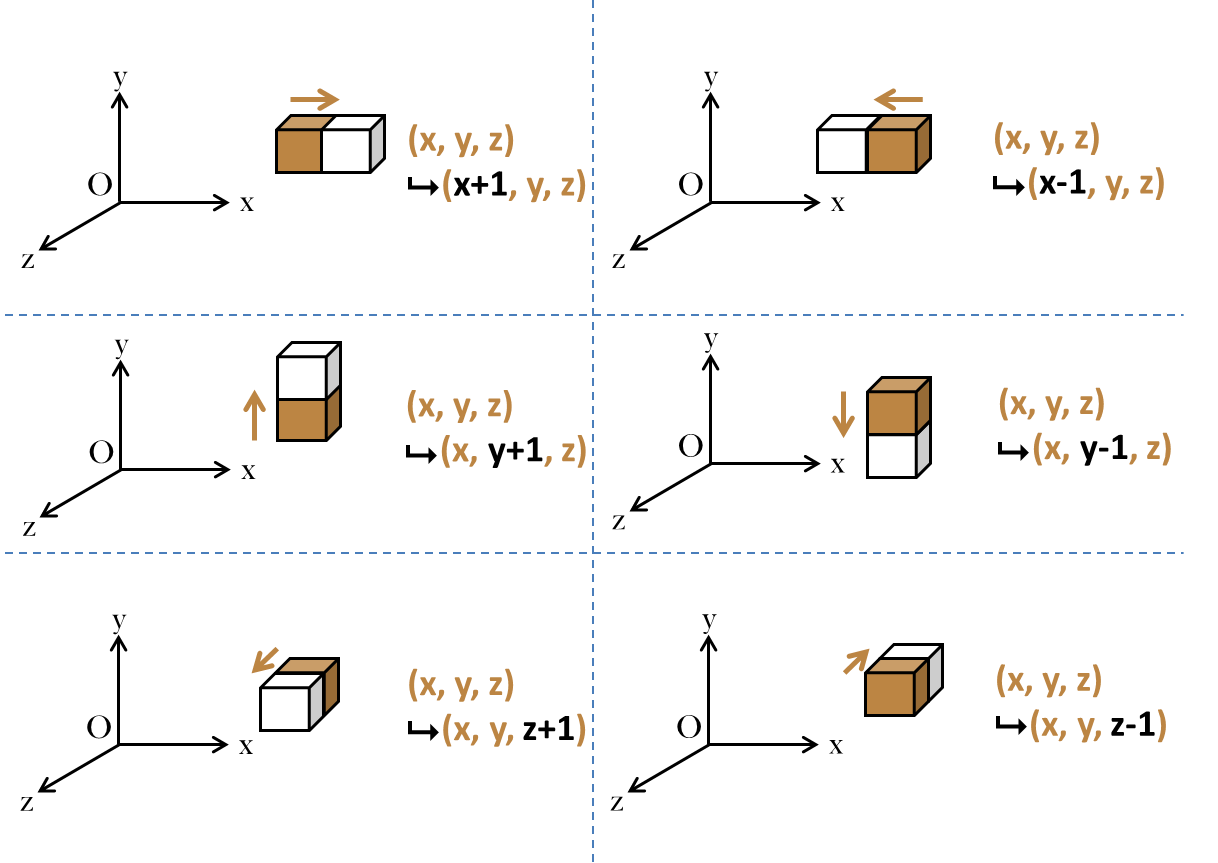
\includegraphics[scale=0.5,keepaspectratio=true]{img/buildChildren.png}
 \caption{Calcul des coordonnées des fils pour six pères différents}
 \label{buildChildren}
\end{figure}

La différence entre les fils d’un nœud intervient lors du calcul de leur direction. Deux cas de figure sont alors à envisager :
\begin{itemize}
 \item le nœud fils correspond à une unité droite (voir figure 4), dans ce cas, un seul nœud fils sera créé et celui-ci héritera de la direction de son père
 \item le nœud fils correspond à un coin, dans ce cas, plusieurs nœuds fils seront créés avec des directions différentes de celle du père
\end{itemize}
 
La figure~\ref{buildCornerChildren} illustre le fonctionnement de l’arbre pour placer la 3e unité du serpent à partir d’un nœud donné. Les flèches indiquent les directions associées au dernier cube placé. À la hauteur n, on a déjà positionné les deux premières unités et la 2e unité a pour direction droite.  Étant donné que la 3e unité est un coin (voir figure 4), il convient que la direction change entre la 2e et la 3e unité. Ainsi, les directions possibles pour la 3e unité sont : bas, derrière, devant et haut, d’où les quatre nœuds représentés à la hauteur n+1. 
NB : on peut d’ores et déjà remarquer que les directions devant et haut vont déboucher sur une configuration interdite car la prochaine unité créée sortira du cube.

\begin{figure}[h]
 \centering
 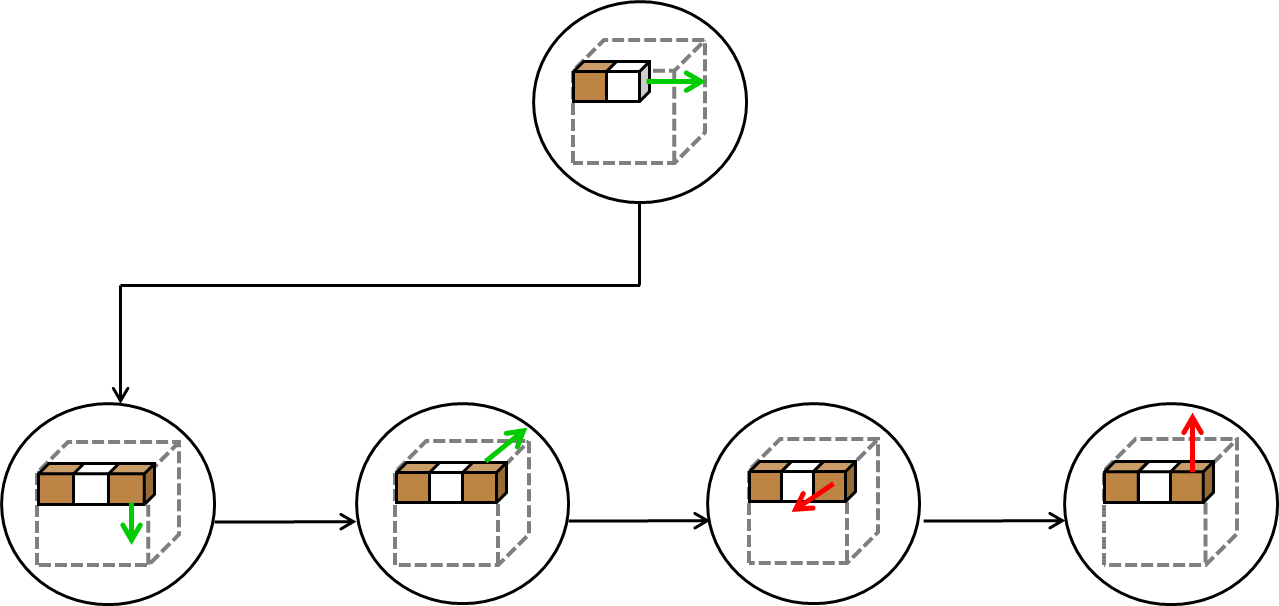
\includegraphics[scale=0.5,keepaspectratio=true]{img/buildCornerChildren.png}
 \caption{Exemple de création des fils pour un coin}
 \label{buildCornerChildren}
\end{figure}

\clearpage
\section{Problème des nœuds initiaux}
Dans cette partie nous allons exposer la méthode employée pour 	placer la première unité dans le volume final. En effet, la démarche exposée jusqu’ici ne s’applique pas pour les premiers nœuds de l’arbre étant donné qu’elle dépend du nœud père. Ici l’enjeu est double puisqu’il faut également déterminer et éliminer les couples coordonnées-direction symétriques. Afin de simplifier la lecture, les couples coordonnées-direction seront appelés vecteurs dans ce qui va suivre. La figure~\ref{startingPoint} illustre en partie le problème des symétries sur la première face du cube. Dans cet exemple, l’unité marron amènera à la création d’un nœud et les trois autres unités devront être reconnues comme étant redondantes et sans intérêt pour le calcul des solutions. 

\begin{figure}[h]
 \centering
 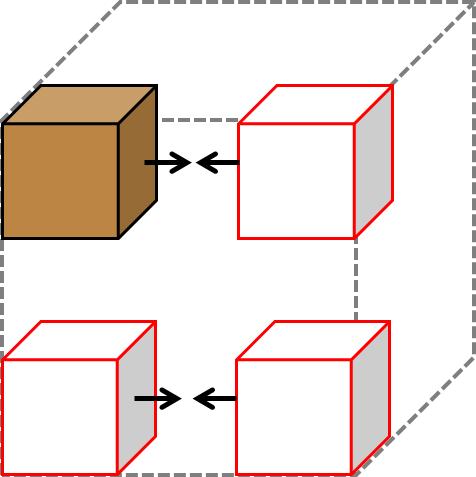
\includegraphics[scale=0.5,keepaspectratio=true]{img/startingPoint.png}
 \caption{Quatre vecteurs initiaux redondants}
 \label{startingPoint}
\end{figure}

La recherche des vecteurs initiaux se déroule en plusieurs étapes et se base sur les axes de symétrie horizontale, verticale et diagonale (en slash et antislash). Il faut d’abord déterminer, parmi ces axes, ceux que l’on peut appliquer aux faces du volume final. Cette information sera fournie dans un fichier contenant les caractéristiques du volume. Une fois les axes connus, nous allons traiter des tranches de volume les unes après les autres. Par tranche on entend l’ensemble des unités appartenant au même plan parallèle à (O ; x, y). Ensuite il convient de projeter orthogonalement le centre géométrique de la figure sur la face en cours de traitement. Une fois les coordonnées du projeté connues, on peut calculer les équations cartésiennes des axes de symétries et ainsi éliminer les vecteurs redondants. Aussi notons que les vecteurs avec une direction qui sort du volume ne seront pas retenus. En suivant ce principe, la recherche des vecteurs initiaux pour un volume cubique 3x3x3 amène à la création de six vecteurs au lieu des cent huit présents.